% Typestate Programming

\begin{frame}[fragile,t]{Typestate Programming 1}
    Den State mit dem Typ darstellen.
    \note<1>{
        Ein Konzept mit der State über den Typ einer variable dargestellt wird. \\
        So können die verschiedenen States und deren Übergänge viel besser Kontrolliert(eingeschränkt) werden. \\
        Es können sich auch die verfügbaren Methoden je nach State ändern.
    }

    \pause Beispiel:
    \begin{figure}
        \centering
        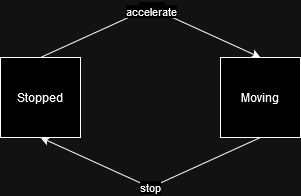
\includegraphics{images/typestate.drawio}
        \caption{Typestate Visualisierung}
        \label{fig:typestate-programming-1}
    \end{figure}

    \note<2>{
        Hier sehen wir das Konzept Visualisiert \\
        Wir haben zwei States: Stopped Moving \\
        Stopped ist der initial-State der mit new() erstellt werden kann \\
        Danach kann mit accelerate und stop_after kontrolliert zwischen den States gewechselt werden
    }

\end{frame}

\begin{frame}[fragile,t]{Typestate Programming 2}
    State "Stopped" initialisieren:
    \begin{lstlisting}[language=Rust,escapechar=@,label={lst:typestate-programming-2-1}]
let car_state: Stopped = Stopped::new();
println!("Starting at {} m", car_state.get_distance());
\end{lstlisting}
    \codeoutput{code/04-typestate1.txt}

    \note<1>{
        Hier sehen wir wie mit der associatierten Funktion "new" eine instanz von Stopped erstellt wird \\
        Initial hat Stopped immer eine distance von 0, die Distanz kann nur durch den wechsel durch die States angepasst werden
    }

    \pause zu State "Moving" übergehen
    \begin{lstlisting}[language=Rust,escapechar=@,label={lst:typestate-programming-2-2}]
let new_car_state: Moving = car_state.accelerate(
    5, // acceleration in m/s^2
    2 // how long to accelerate in seconds
);
println!("Accelerated to {} m/s", new_car_state.get_velocity());
\end{lstlisting}
    \codeoutput{code/04-typestate2.txt}

    \note<2> {
        Stopped hat die Funktion "accelerate", welche eine Instanz von "Moving" zurückgibt \\
        Dies ist der einzige Weg wie der State "Moving" erreicht werden kann \\
        Moving hat eine geschwindigkeit, die ausgelesen werden kann
    }
\end{frame}



\begin{frame}[fragile,t]{Typestate Programming 3}
    zurück zum State "Stopped"
    \begin{lstlisting}[language=Rust,escapechar=@,label={lst:typestate-programming-3-1}]
let final_car_state: Stopped = new_car_state.stop_after(
    10 // after how many seconds to stop moving
);

println!("Reached destination at {} m", final_car_state.get_distance());
    \end{lstlisting}
    \codeoutput{code/04-typestate3.txt}

    \note{
        Schlussendlich kann mit stop_after wieder zum State Stopped zurückgekehrt werden \\
        Jetzt hat sich die Distanz erhöht, da für eine gewisse Zeit mit einer gewissen Geschwindigkeit bewegt wurde \\
        Die kann in Rust sehr einfach implementiert werden, da die Typisierung strict ist \\
        Dadurch dass es keine Vererbung gibt, kann auch nicht einfach ein CustomMoving State erstellt werden
    }
\end{frame}
